\chapter{Background}

\section{Quantum Information and Entanglement}

This section will focus on the basics of quantum information that are relevant to understanding the Bell basis distinguishability question for LELM devices.

\subsection{Bits, Qubits, Qutrits, Qudits}

% Bits and Qubits

The basic unit of classical information is the bit, which can take on either the value $0$ or $1$. A bit is exactly enough information necessary to describe the state of a two-state system. A common example is that of a light-switch, for which $0$ could represent ``off'' and $1$ could represent ``on.''

The quantum analog of the bit is the \textit{qubit}. Qubits also describe two-state systems; however, they allow for specific combinations of possibilities. Qubits can take on either the value $\ket{0}$, $\ket{1}$, or any value of the form
\[
\ket{b} = \alpha \ket{0} + \beta \ket{1}
\]
where $\alpha$ and $\beta$ are complex numbers normalized such that $|\alpha|^2 + |\beta|^2 = 1$. The notation $\ket{}$ is called a \textit{ket}. Another way to represent the same qubit is as a column vector
\[b = 
\begin{pmatrix}
	\alpha \\
	\beta
\end{pmatrix}
\]
but the ket notation is often more efficient. 

When one wishes to collect a value from a qubit, they \textit{measure} it. Then the qubit `collapses' and unambiguously become either $\ket{0}$ or $\ket{1}$. The probability of the qubit collapsing to each state are determined by $\alpha$ and $\beta$, with probability $|\alpha|^2$ of collapsing to $\ket{0}$ and probability $|\beta|^2$ of collapsing to $\ket{1}$.

% Bases

The set of all possible values for a qubit is a vector space of dimension two. One basis for this space is $\{\ket{0}, \ket{1}\}$. Measurements can be performed in any orthogonal basis. Other common orthogonal bases include
\[
\left\{\frac{1}{\sqrt{2}}\ket{0} + \frac{1}{\sqrt{2}}\ket{1}, \; \frac{1}{\sqrt{2}}\ket{0} -\frac{1}{\sqrt{2}} \ket{1}\right\}
\] and
\[
\left\{\frac{1}{\sqrt{2}}\ket{0} + \frac{i}{\sqrt{2}}\ket{1}, \; \frac{1}{\sqrt{2}}\ket{0} -\frac{i}{\sqrt{2}} \ket{1}\right\}.
\] If a qubit $\ket{b}$ is measured in the orthogonal basis $\{\ket{x}, \ket{y}\}$, then there is a $|\braket{b}{x}|^2$ probability of measuring $\ket{x}$ and a $|\braket{b}{y}|^2$ probability of measuring $\ket{y}$.   Here, we've used the notation $\braket{b}{x}$ to represent the inner product of $\ket{b}$ and $\ket{x}$. Moreover, the symbol $\bra{}$ is called a \textit{bra}, and it is used to represent the conjugate transpose of a ket.  Hence, the conjugate transpose of the `column' vector $\frac{1}{\sqrt{2}}\ket{0} -\frac{i}{\sqrt{2}} \ket{1}$ would be the `row' vector $\frac{1}{\sqrt{2}}\bra{0} + \frac{i}{\sqrt{2}} \bra{1}$. 


% Qtrits and Qdits

Sometimes---such as in this thesis---we have the desire to represent systems that can take on more than two states. \textit{Qutrits} represent systems that can take on three values, and \textit{qudits} are refer to the generalizations of qubits that represent systems with an arbitrary (but finite) number of states. We write an arbitrary qutrit as 
\[
\ket{t} = \alpha \ket{0} + \beta \ket{1} + \gamma \ket{2}
\]
and an arbitrary qudit as
\[
\ket{q} = \alpha_0 \ket{0} + \alpha_1 \ket{1} + \cdots + \alpha_{d-1} \ket{d-1}.
\] The numerical labels inside the kets can of course be changed without affecting any of the physics or the math.

% Multi-particle systems

Another useful generalization to consider is that of multi-particle systems. In classical computing, two-bit systems can take on four values: $00$, $01$, $10$, and $11$. In the notation of quantum information, we write these four values as: 
\[
\ket{0} \otimes \ket{0}, \ket{0} \otimes \ket{1}, \ket{1} \otimes \ket{0}, \text{ and } \ket{1} \otimes \ket{1}.
\] The $\otimes$ symbol is used because our $\ket{0}$ and $\ket{1}$ kets are vectors, and their product in an element of a tensor product space. Similarly to how a qubit can be an arbitrary normalized linear combination of $\ket{0}$ and $\ket{1}$, states in a multi-particle system can be any normalized linear combination of the vectors $\ket{0} \otimes \ket{0}, \ket{0} \otimes \ket{1}, \ket{1} \otimes \ket{0}, \text{ and } \ket{1} \otimes \ket{1}$. Often we will omit the $\otimes$ and write $\ket{0} \otimes \ket{0}$ as either $\ket{0} \ket{0}$ or as $\ket{00}$.


\subsection{Entanglement}

Entanglement refers to any multi-particle quantum state that cannot be represented as 

Two examples of non-entangled quantum states are $\ket{11}$ and $\frac{1}{\sqrt{2}}\ket{11}$


A state is maximally entangled if knowing information about one 


% How to check if a state is fully entangled 

% density matrix, etc....

\subsection{The Basics of Bell Bases}

The canonical Bell basis consists of the four states:

\begin{align*}
	\ket{\Phi^+} &= \frac{1}{\sqrt{2}} \pn{\ket{0}\ket{0} + \ket{0}\ket{0}} \\
	\ket{\Phi^-} &= \frac{1}{\sqrt{2}} \pn{\ket{0}\ket{0} - \ket{0}\ket{0}} \\
	\ket{\Psi^+} &= \frac{1}{\sqrt{2}} \pn{\ket{0}\ket{1} + \ket{1}\ket{0}} \\
	\ket{\Psi^-} &= \frac{1}{\sqrt{2}} \pn{\ket{0}\ket{1} - \ket{1}\ket{0}}
\end{align*}

The Bell basis is a basis of entangled states for a two-particle system. If each particle has dimension $d$, then the Bell basis is:
\[
\left\{ \ket{\Psi_c^p} = \frac{1}{\sqrt{d}} \sum_{j=0}^{d-1} \omega^{pj} \ket{j}\ket{j + c \;(\text{mod}\; d)} \text{ such that } c, p \in \mathbb{Z} \text{ and } 0 \leq c,p < d \right\}
\]
where $\omega = e^{i 2 \pi / d}$ is a primitive $d$th root of unity. Thus, for two $d$-dimensional particles, there are $d^2$ states in the Bell basis.

\section{Linear Evolution Local Measurement Apparatuses}

A Linear Evolution Local Measurement (LELM) apparatus (Figure \ref{fig:apparatus}) has two main parts to it. The Linear Evolution part of the LELM apparatus refers to how the device can linearly evolve either particle separately, but cannot manipulate a particle based on the value of the other. So, for example, LELM devices cannot perform a controlled bit-shift. The Local Measurement part of the LELM apparatus refers to how measurements are restricted to acting on a single particle at a time. Thus, a LELM apparatus takes in two particles, and outputs two detection events or `clicks'.

\begin{figure}
\centering
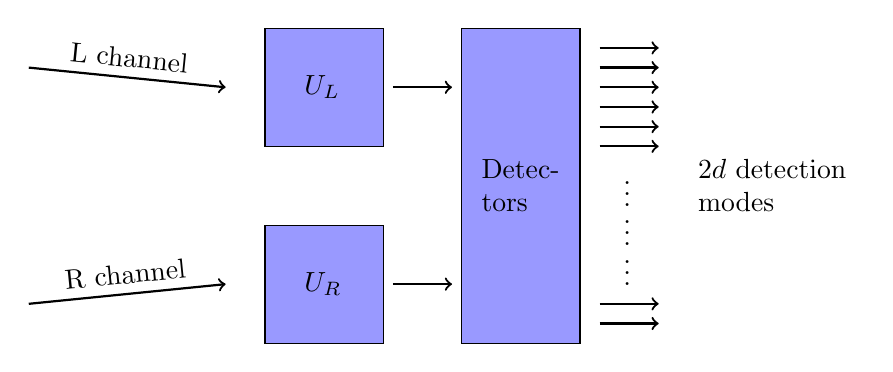
\begin{tikzpicture}
\filldraw[fill=blue!40!white, draw=black] (2.5,0) rectangle (4,4);
\filldraw[fill=blue!40!white, draw=black] (0,0) rectangle (1.5,1.5);
\filldraw[fill=blue!40!white, draw=black] (0,2.5) rectangle (1.5,4);
\draw[thick,->] (-3,3.5) -- (-0.5,3.25) node[midway, above, sloped] {L channel};
\draw[thick,->] (-3,0.5) -- (-0.5,0.75) node[midway, above, sloped] {R channel};
\node[text width=3cm] at (2, 0.75) {$U_{\text{R}}$};
\node[text width=3cm] at (2, 3.25) {$U_{\text{L}}$};
\node[text width=1cm] at (3.25, 2) {Detec- tors};

\draw[thick,->] (1.625,3.25) -- (2.375,3.25);
\draw[thick,->] (1.625,0.75) -- (2.375,0.75);

\draw[thick,->] (4.25,3.75) -- (5,3.75) node[midway, above] {};
\draw[thick,->] (4.25,3.5) -- (5,3.5) node[midway, above] {};
\draw[thick,->] (4.25,3.25) -- (5,3.25) node[midway, above] {};
\draw[thick,->] (4.25,3.0) -- (5,3.0) node[midway, above] {};
\draw[thick,->] (4.25,2.75) -- (5,2.75) node[midway, above] {};
\draw[thick,->] (4.25,2.5) -- (5,2.5) node[midway, above] {};
\node (A) at (4.6,2) {$\vdots$};
\node (A) at (4.6,1.5) {$\vdots$};
\node (A) at (4.6,1) {$\vdots$};
\draw[thick,->] (4.25,0.5) -- (5,0.5) node[midway, above] {};
\draw[thick,->] (4.25,0.25) -- (5,0.25) node[midway, above] {};
\node[text width=2cm] (A) at (6.5,2) {$2d$ detection modes};
\end{tikzpicture}
\caption{A LELM apparatus.} \label{fig:apparatus}
\end{figure}

The basis of single-particle states is:
\[
\mathcal{B}_{\text{single-particle}} = \{\ket{0, L}, \ket{0, R}, \ket{1, L}, \ket{1, R}, \ldots, \ket{d-1, L}, \ket{d-1, R}\}
\]
The basis is of size $2d$, since each particle can either be from the left channel or the right channel.

A pair of two detector modes is called a detection signature. Each detection mode is an element in the span of $\mathcal{B}_{\text{single-particle}}$. However, if $\ket{i}$ and $\ket{j}$ are detection modes then when determining their combined detection signature, we cannot simply take $\ket{i} \otimes \ket{j}$, since that may include inputs where two particles are coming from the same channel. Thus, we introduce the $P_{LR}$ projection operator, which removes all elements of $\mathcal{B}_{\text{single-particle}} \times \mathcal{B}_{\text{single-particle}}$ of the form $\ket{*, L}\ket{*', L}$ or $\ket{*, R}\ket{*', R}$ and renormalizes resulting the state.

\section{The Distinguishability Problem}

\subsection{Motivation}
\subsection{Formalization}